\subsection{Design, comparators and service endpoints}
We evaluate whether [EL], [AU] and [SUP] jointly preserve legal progress
under unchanged selected feedback histories. Core factorial controls
separate computation retention from whole-view retention; native tests
measure confirmed full calls executing the original correction task.
An instrumented FIFO Consumer records actual applications. All accepted
inputs keep their original ready times through cancellation and recovery.

\paragraph{Core implementation and sources}
Two 24-GB RTX~3090s host an FP16 Private worker and FP32 Authority worker.
Qwen3-ASR~1.7B~\cite{shi2026qwen3asr} is primary; Whisper base.en
\cite{radford2023whisper} tests a second state adapter. Complete-row
delivery, at most 16 rows per batch, a 256-token limit, the protocol kernel
and synchronized journals are shared. Physical early exit is disabled
in this factorial study, separating retention from cancellation.
Initial loading precedes the service clock. Energy integrates both
physical boards over the declared service window.

Independent confirmation uses 24 previously unused LibriSpeech speakers
\cite{panayotov2015librispeech}, metadata-selected before inference and
partitioned into three eight-speaker cohorts, totaling 714.110~s per arm.
Its 110 cells comprise 60 primary cells (three cohorts, two backends, two
arrival patterns, five arms), 20 fresh-process repeats on cohort~A and 30
coarser-feedback controls. At $\rho=1$, Authority advances every 2~s;
$\rho=3$ changes selection frequency and feedback segmentation. Arrivals
are simultaneous or staggered by 0.25~s. Repetitions and arms reuse these
sources; speakers are the independent acoustic units.

\paragraph{Named comparisons}
\emph{Checked snapshot + recomputation} ($R_0S_0$), \emph{View retention
only} ($R_0S_1$), \emph{Computation retention only} ($R_1S_0$), and
\emph{RevTrace: joint retention} ($R_1S_1$) share validation, durability,
input accounting and physical execution. Disabling $R$ rebuilds work
from selected feedback; disabling $S$ replaces the provisional view
with the installed snapshot while retaining the same dependency checks.
The \emph{Alternative joint implementation} is our complete positive
control: another policy instantiation of the same retention and Consumer
conditions on the shared execution/commit substrate. External prior work
and our author-built comparators have separate identities.

\paragraph{Endpoints}
For offered interval $i$, $w_i$ is audio duration, $r_i$ its original
ready time, $d_i$ first actual visible coverage and $c_i$ first actual
certified coverage. Audio coverage meeting both deadlines is
\begin{equation}
 A_{2,8}=\sum_i w_i\,\mathbf{1}
 \{d_i-r_i\leq2\ \land\ c_i-r_i\leq8\}.
 \label{eq:credit}
\end{equation}
All offered intervals, including partial end-of-stream (EOS) tails,
remain in the denominator. Whole-run passes require display P99 at most
2~s (D2) and certified-view P99 at most 8~s (C8), over offered frontiers.
P99 weights frontier observations; $A_{2,8}$ weights duration, so a P99
pass may coexist with a small uncredited tail.

We separately count visible-frontier withdrawals, erased code points and
deficit below the previously observed frontier. Retrospective whole-text
support compares a first actual view with later selected text at that
view's own frontier. This is distinct from dependency validity [SUP],
human word/character error rate, and new character count. Independent
checks reconstruct complete selected $F/Z/P/\mathrm{text}$ histories and
actual consumed input paths from original outputs.

\subsection{Does retaining computation retain delivered service?}
Retaining computation alone can improve timeliness while increasing
withdrawal. Figure~\ref{fig:main_evidence}(a) shows the predeclared Qwen,
$\rho=1$, staggered stratum. With the same selected histories, computation
retention raises covered audio from 654.115 to 664.150~s but withdrawals
from 12 to 17. View retention alone reduces withdrawals to 1 but covers
628.435~s. RevTrace jointly covers 680.760~s with zero frontier withdrawals:
26.645~s above recomputation and 16.610~s above computation-only.

\begin{figure*}[t]
\centering
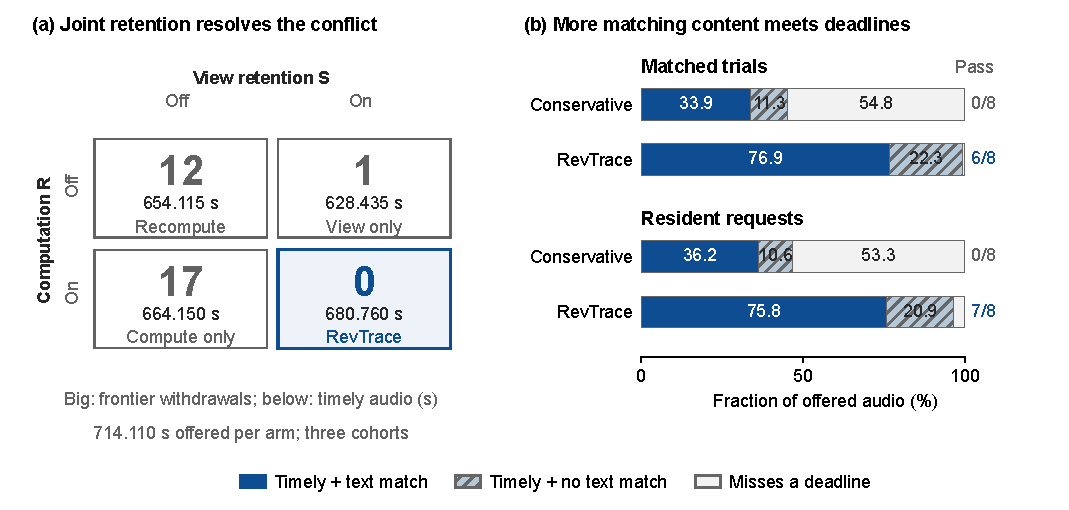
\includegraphics[width=\textwidth]{figures/joint_and_content.pdf}
\caption{Retained work and retained service require coordinated decisions.
(a) The predeclared 24-speaker stratum: each cell sums three eight-speaker cohorts'
frontier withdrawals and audio coverage meeting display 2~s/certified 8~s
deadlines over 714.110~s per arm. The four matrix arms and our separate
Alternative joint positive control (15 runs total)
fail whole-run D2. (b) Final native matched and resident banks each offer
66.340~s per policy on four existing sources. Stacks separate timely
same-frontier whole-text agreement, other timely coverage and uncovered
audio; text agreement is retrospective against selected model output.
Unlabelled tails are the remainder to 100\%, with rounded labels.
Passes count matched trials or resident requests meeting display P99
$\leq2$~s and certified P99 $\leq8$~s.}
\label{fig:main_evidence}
\end{figure*}

Cohort-wise credit interaction,
$I=Y_{11}-Y_{10}-Y_{01}+Y_{00}$, is $+18.530$, $+6.205$, and $+17.555$~s.
These are three queue-coupled cohort contrasts, not independent deadline
windows. RevTrace's text remains revisable: 569 characters are erased
despite zero frontier withdrawal. Median per-run display P99 is 2.329~s,
above D2, so the benefit is retained progress under overload rather than
a whole-run service pass.

The Alternative joint implementation also yields zero withdrawals and 569
erased characters, with 667.530~s coverage and 2.534-s median P99. It
reproduces the supported-view behavior on the common substrate. Across
confirmation, 144 matched history groups and 22 positive-control pairs
agree on complete selected histories. Thus the comparison holds the
feedback task fixed while changing how valid work becomes service.
\par\noindent\textbf{Finding 1: retained computation does not ensure retained service.}
[EL] can retain work whose presentation a snapshot Consumer still removes.
Joint [EL]/[SUP] coordination preserves the supported ahead view.
